%! TEX program = pdflatex

\documentclass[oneside,solution]{karazin-complan-assign}

\usepackage[utf8]{inputenc}
\usepackage[english,ukrainian]{babel}

\usepackage{mathtools}

\let\Im\relax
\DeclareMathOperator{\Im}{Im}
\let\Re\relax
\DeclareMathOperator{\Re}{Re}

\usetikzlibrary{decorations.markings,positioning}

\providecommand{\poles}{
  \node (poles) at (2.5,1.5) {poles of $h(p_0)$};
  \draw[fill]
  (1.5,3) coordinate [circle,fill,inner sep=1pt,label=right:$p_1$] (p1)
  (2,-2) coordinate [circle,fill,inner sep=1pt,label=below:$p_2$] (p2)
  (-3,1) coordinate [circle,fill,inner sep=1pt,label=above:$p_3$] (p3)
  (-2,-1.5) coordinate [circle,fill,inner sep=1pt,label=above:$p_4$] (p4);
  \draw[ultra thin,gray] (poles) -- (p1) (poles) -- (p2) (poles.west) -- (p3) (poles) -- (p4);
}

\def\xr{3.5}
\def\yr{3}


\title{Домашня робота}
\author{Захаров Дмитро}
\studentID{МП-31}
\instructor{Гиря Н.П.}
\date{\today}
\duedate{23:59 14 квітня, 2024}
\assignno{3}
\semester{Весняний семестр 2024}
\mainproblem{Обчислення Інтегралів \#2. Варіант 5}

\begin{document}

\maketitle

% \startsolution[print]

\problem{}

\textbf{Умова.} Обчислити інтеграл
\begin{equation*}
    \mathcal{I} = \int_{-\infty}^{+\infty} \frac{e^{-2ix}x^2dx}{(x^2+4ix-5)^2}
\end{equation*}

\textbf{Розв'язання.} Введемо допоміжний контур (див. Рисунок \ref{fig:contour_1}):
\begin{equation}
    \gamma = \underbrace{[-R, R]}_{\xleftarrow{}} \cup C_R, \; C_R := \{z \in \mathbb{C}: |z|=1 \wedge \text{Im}(z) < 0\},
\end{equation}

де $C_R$ -- нижнє півколо радіусу $R$. Також позначимо $\mathcal{I}_{\gamma} = \oint_{\gamma} f(z)dz$ де
\begin{equation}
    f(z) = \frac{e^{-2iz}z^2}{(z^2+4iz-5)^2}.
\end{equation}

В такому разі з нашого розбиття маємо:
\begin{equation}
    \mathcal{I}_{\gamma} = -\int_{-R}^{+R} f(x)dx + \int_{C_R} f(z)dz 
\end{equation}

Якщо взяти граничний перехід при $R \to +\infty$:
\begin{equation}
    \mathcal{I}_{\gamma} = -\mathcal{I} + \lim_{R \to \infty} \int_{C_R} f(z)dz
\end{equation}

Ідея наступна: нам потрібно спочатку знайти $\mathcal{I}_{\gamma}$, а потім довести, що $\lim_{R \to \infty}\int_{C_R}f(z)dz=0$, з чого ми знаходимо шуканий інтеграл $\mathcal{I} = -\mathcal{I}_{\gamma}$. 

\begin{figure}
    \centering
    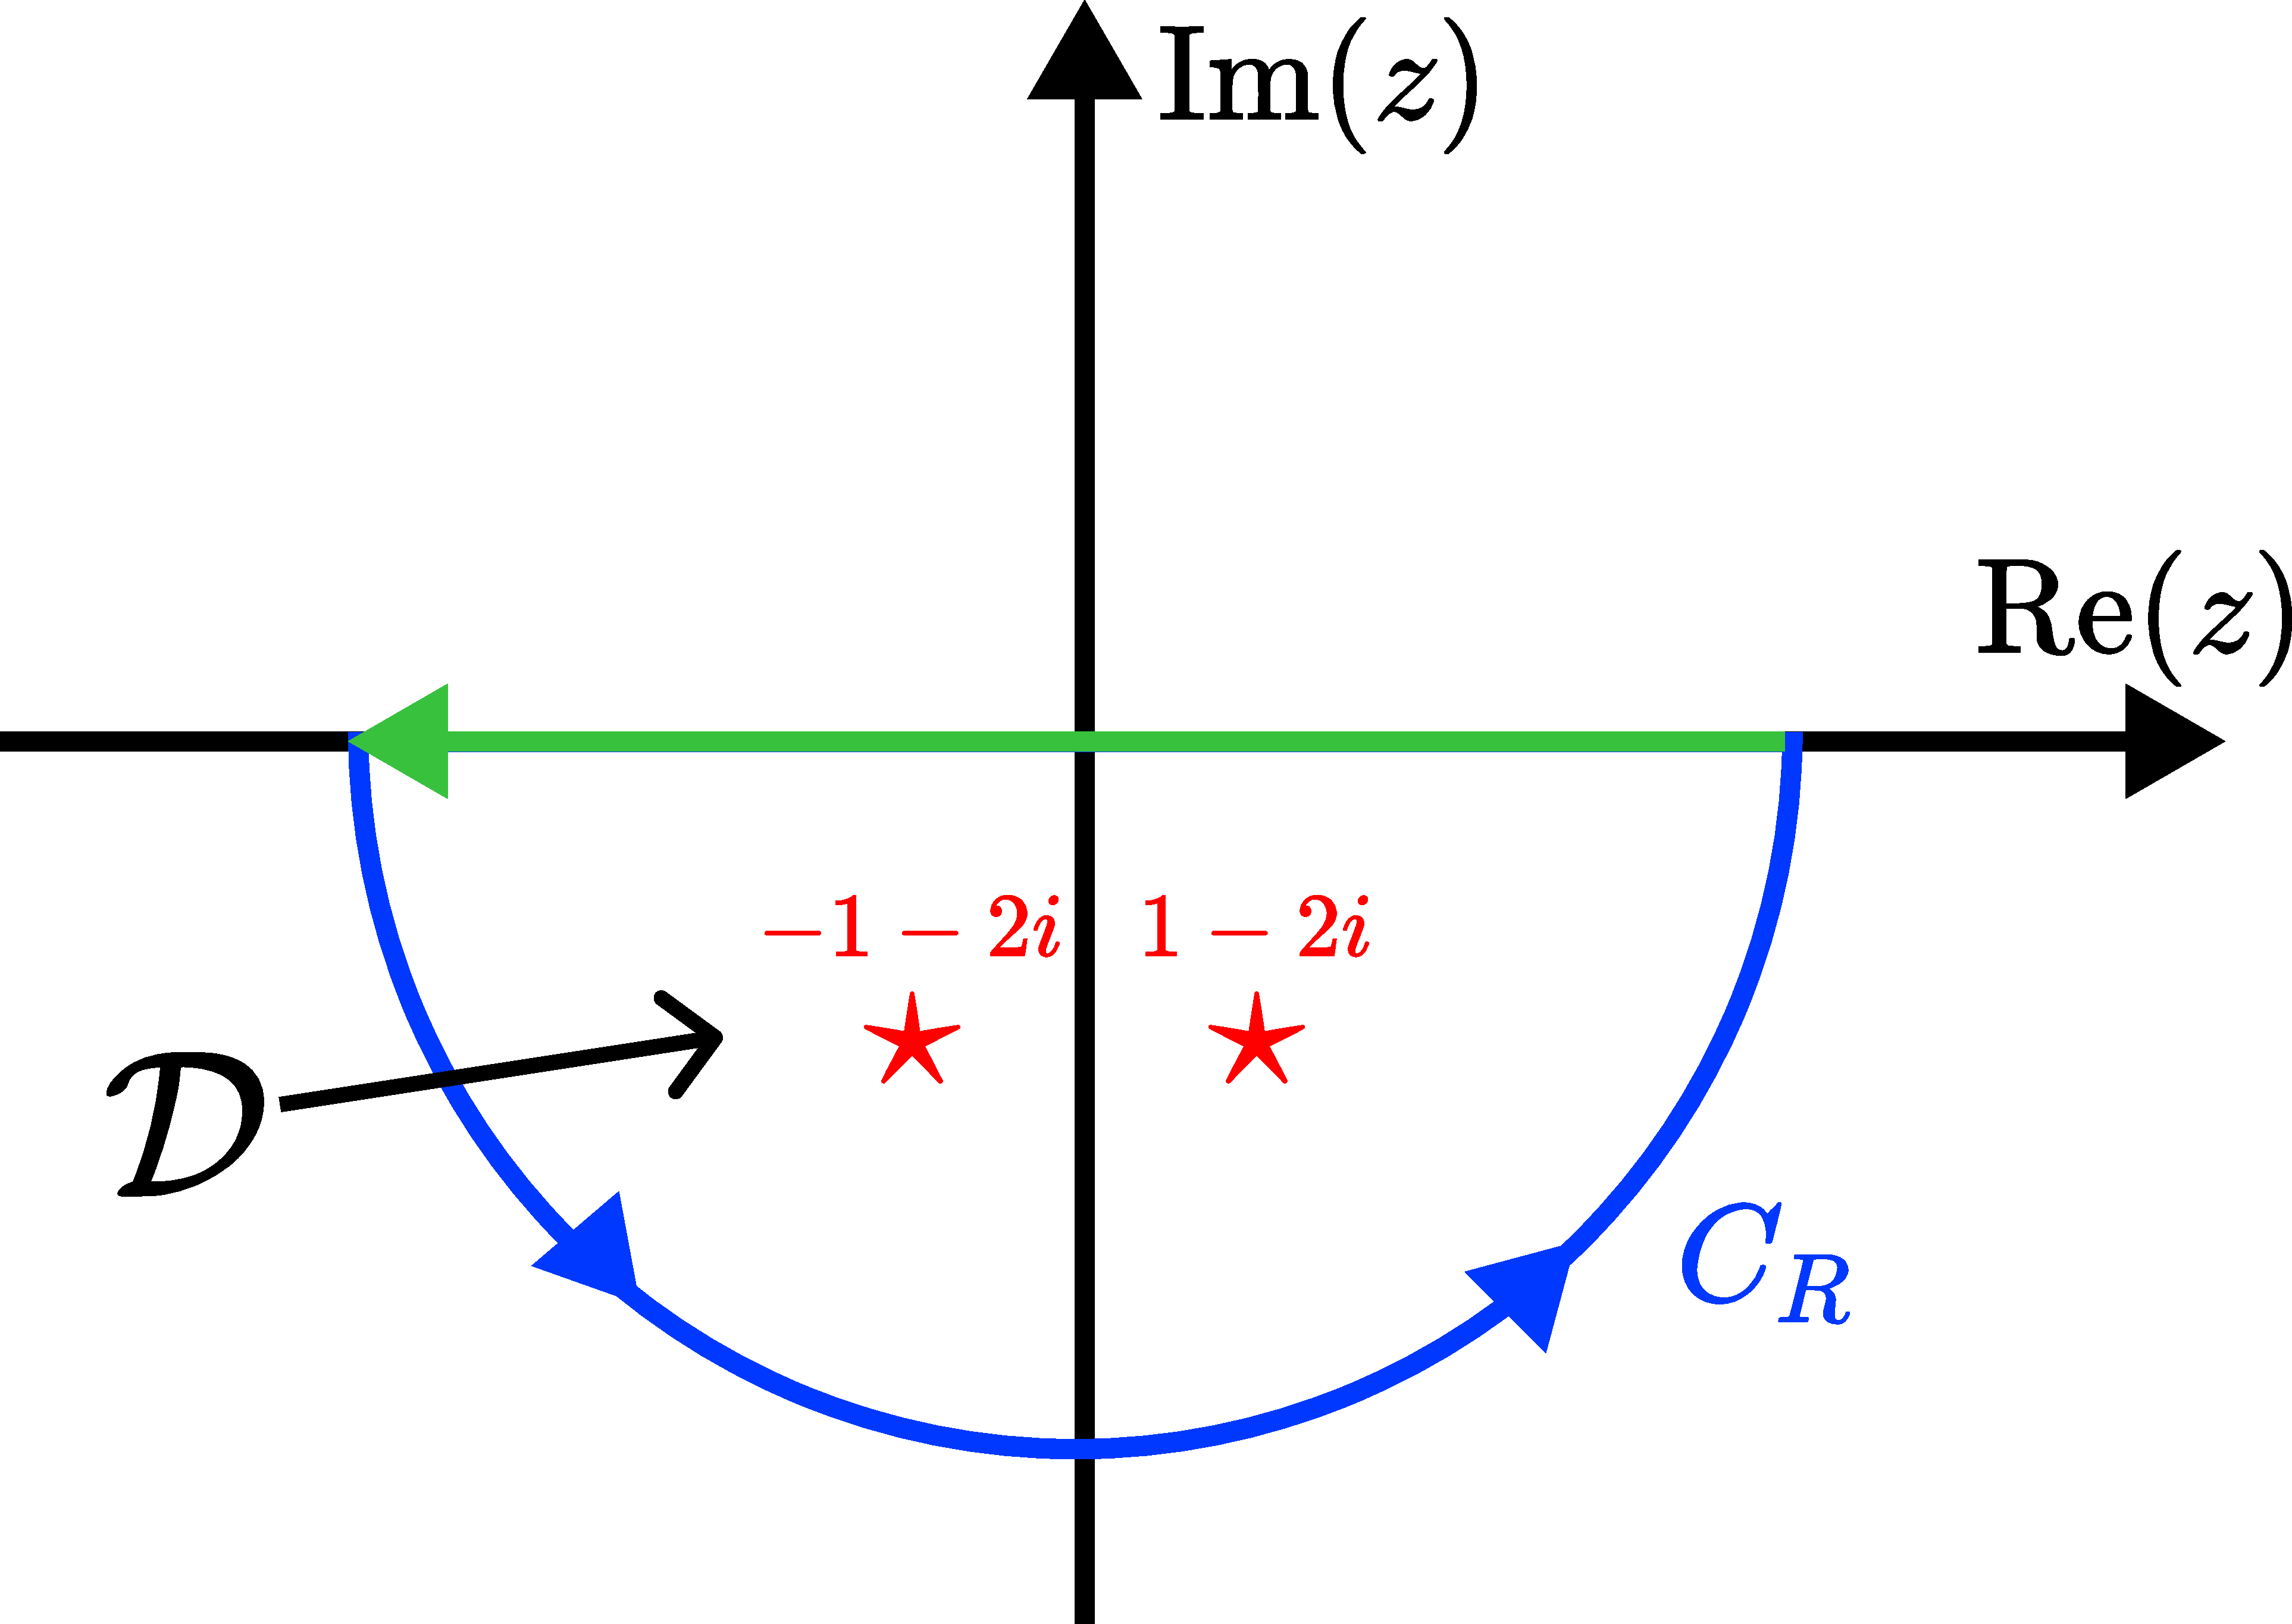
\includegraphics[width=0.6\textwidth]{images/hw_3/contour_1.pdf}
    \caption{Контур $\gamma$ в задачі 1 з особливими точками $f(z)$.}
    \label{fig:contour_1}
\end{figure}

\textbf{Крок 1. Обчислення допоміжного інтегралу.} Для цього спочатку знайдемо особливі точки. Для цього прирівнюємо до нуля поліном в знаменнику:
\begin{equation}
    z^2 + 4iz - 5 = 0 \implies z = -1 - 2i, \; z = 1-2i
\end{equation}

Отже, маємо дві особливі точки -- $z_1=-1-2i$ та $z_2=1-2i$. Обидві точки є полюсом другого порядку (оскільки поліном додатково стоїть у другій ступені), причому обидві належать області $\mathcal{D}$ ($\partial\mathcal{D} = \gamma$). Тому,
\begin{equation}
    \mathcal{I}_{\gamma} = 2\pi i (\text{Res}_{z=z_1}f(z) + \text{Res}_{z=z_2}f(z))
\end{equation}

Знайдемо лишки:
\begin{gather}
    \text{Res}_{z=z_1}f(z) = \lim_{z \to z_1} ((z-z_1)^2 f(z))' = \lim_{z \to z_1} \frac{d}{dz}\frac{e^{-2iz}z^2}{(z-z_2)^2} \nonumber \\ 
    = \lim_{z \to z_1} \frac{(-2ie^{-2iz}z^2 + 2ze^{-2iz})(z-z_2)^2 - 2(z-z_2)e^{-2iz}z^2}{(z-z_2)^4} \nonumber \\
    = \lim_{z \to z_1}\frac{2ze^{-2iz}\left((1-iz)(z-z_2) - z\right)}{(z-z_2)^3} \nonumber \\
    = \lim_{z \to z_1} \frac{2ze^{-2iz}(izz_2-z_2-iz^2)}{(z-z_2)^3} \nonumber \\
    = \frac{2z_1e^{-2iz_1}(iz_1z_2-z_2-iz_1^2)}{(z_1-z_2)^3} = \left(\frac{3}{4}+\frac{3i}{2}\right)e^{-4+2i}
\end{gather}

Аналогічним чином:
\begin{equation}
    \text{Res}_{z=z_2}f(z) = \frac{2z_2e^{-2iz_2}(iz_1z_2 - z_1 - iz_2^2))}{(z_2-z_1)^3} = \left(-\frac{3}{4}+\frac{3i}{2}\right)e^{-4-2i}
\end{equation}

Отже, остаточно маємо:
\begin{equation}
    \mathcal{I}_{\gamma} = 2\pi i \left(\left(\frac{3}{4}+\frac{3i}{2}\right)e^{-4+2i} + \left(-\frac{3}{4}+\frac{3i}{2}\right)e^{-4-2i}\right)
\end{equation}

Цей вираз можна дещо спростити, якщо врахувати той факт, що $e^{-4+2i}=e^{-4}(\cos 2 + i \sin 2)$, а $e^{-4-2i}=e^{-4}(\cos 2 - i \sin 2)$:
\begin{equation}
    \mathcal{I}_{\gamma} = -\frac{3\pi(2 \cos 2 + \sin 2)}{e^4}.
\end{equation}

\textbf{Крок 2. Оцінка інтегралу.} Тепер доведемо, що $\lim_{R \to \infty}\int_{C_R}f(z)dz=0$. Для цього помітимо, що
\begin{equation}
    f(z) = e^{-2iz}g(z), \; g(z) = \frac{z^2}{(z^2+4iz - 5)^2}
\end{equation}

А далі скористаємось наслідком \textbf{леми Жордана} для нижнього півкола $C_R$: якщо $f(z)=e^{i\alpha z}g(z)$ і $\alpha<0$, то

\begin{equation}
\lim_{R \to \infty} \sup_{z \in C_R} |g(z)| = 0 \implies \lim_{R \to \infty}\int_{C_R}f(z)dz = 0
\end{equation}

Отже, покажемо, що дійсно $\lim_{R \to \infty} \sup_{z \in C_R} |g(z)| = 0$:
\begin{equation}
    |g(z)| = \frac{|z|^2}{|z^2+4iz-5|^2} = \frac{R^2}{|z-z_1|^2|z-z_2|^2}
\end{equation}

Оцінимо знаменник за допомогою нерівності $|z - w| \geq ||z|-|w||$:
\begin{equation}
    |z-z_1| \geq ||z| - |z_1|| = |R - \sqrt{5}| = R - \sqrt{5} \; \text{(для великих $R$)}
\end{equation}

Аналогічно $|z-z_2| \geq R - \sqrt{5}$. Тому, 
\begin{equation}
    |g(z)| \leq \frac{R^2}{(R-\sqrt{5})^4} \sim \frac{1}{R^2} \xrightarrow[R \to \infty]{} 0
\end{equation}

Отже, звідси отримуємо $\lim_{R \to \infty}\int_{C_R}f(z)dz=0$. Отже, остаточно:
\begin{equation}
    \boxed{\mathcal{I} = \frac{3\pi(2\cos 2 + \sin 2)}{e^4}}
\end{equation}

\textbf{Відповідь.} $\frac{3\pi(2\cos 2 + \sin 2)}{e^4}$. 

\problem{}

\textbf{Умова.} Обчислити інтеграл
\begin{equation*}
    \mathcal{I} = \int_{-\infty}^{+\infty} \frac{e^{\frac{x}{4}}}{4+e^x}dx
\end{equation*}

\textbf{Розв'язання.} В цій задачі спочатку знайдемо особливі точки підінтегральної функції $f(z) = \frac{e^{z/4}}{4+e^z}$. Прирівняємо знаменник до $0$:
\begin{equation}
    e^z = -4 \implies z = \text{Log}(-4) = 2 \log 2 + i\pi + 2\pi i k, \; k \in \mathbb{Z}
\end{equation}

В якості контуру оберемо прямокутник ширини $R$ і висоти $2\pi$. Тоді, наш контур (див. Рисунок \ref{fig:contour_2}):
\begin{equation}
    \gamma = \gamma_x^+ \cup \gamma_y^+ \cup \gamma_x^- \cup \gamma_y^-,
\end{equation}
де $\gamma_x^+$ -- горизональний відрізок від $(-R,0)$ до $(R,0)$, $\gamma_x^-$ -- відрізок від $(R,2\pi)$ до $(-R,2\pi)$, $\gamma_y^+$ -- вертикальний відрізок від $(R,0)$ до $(R,2\pi)$, а $\gamma_y^-$ -- вертикальний відрізок від $(-R,2\pi)$ до $(-R,0)$. 

\begin{figure}
    \centering
    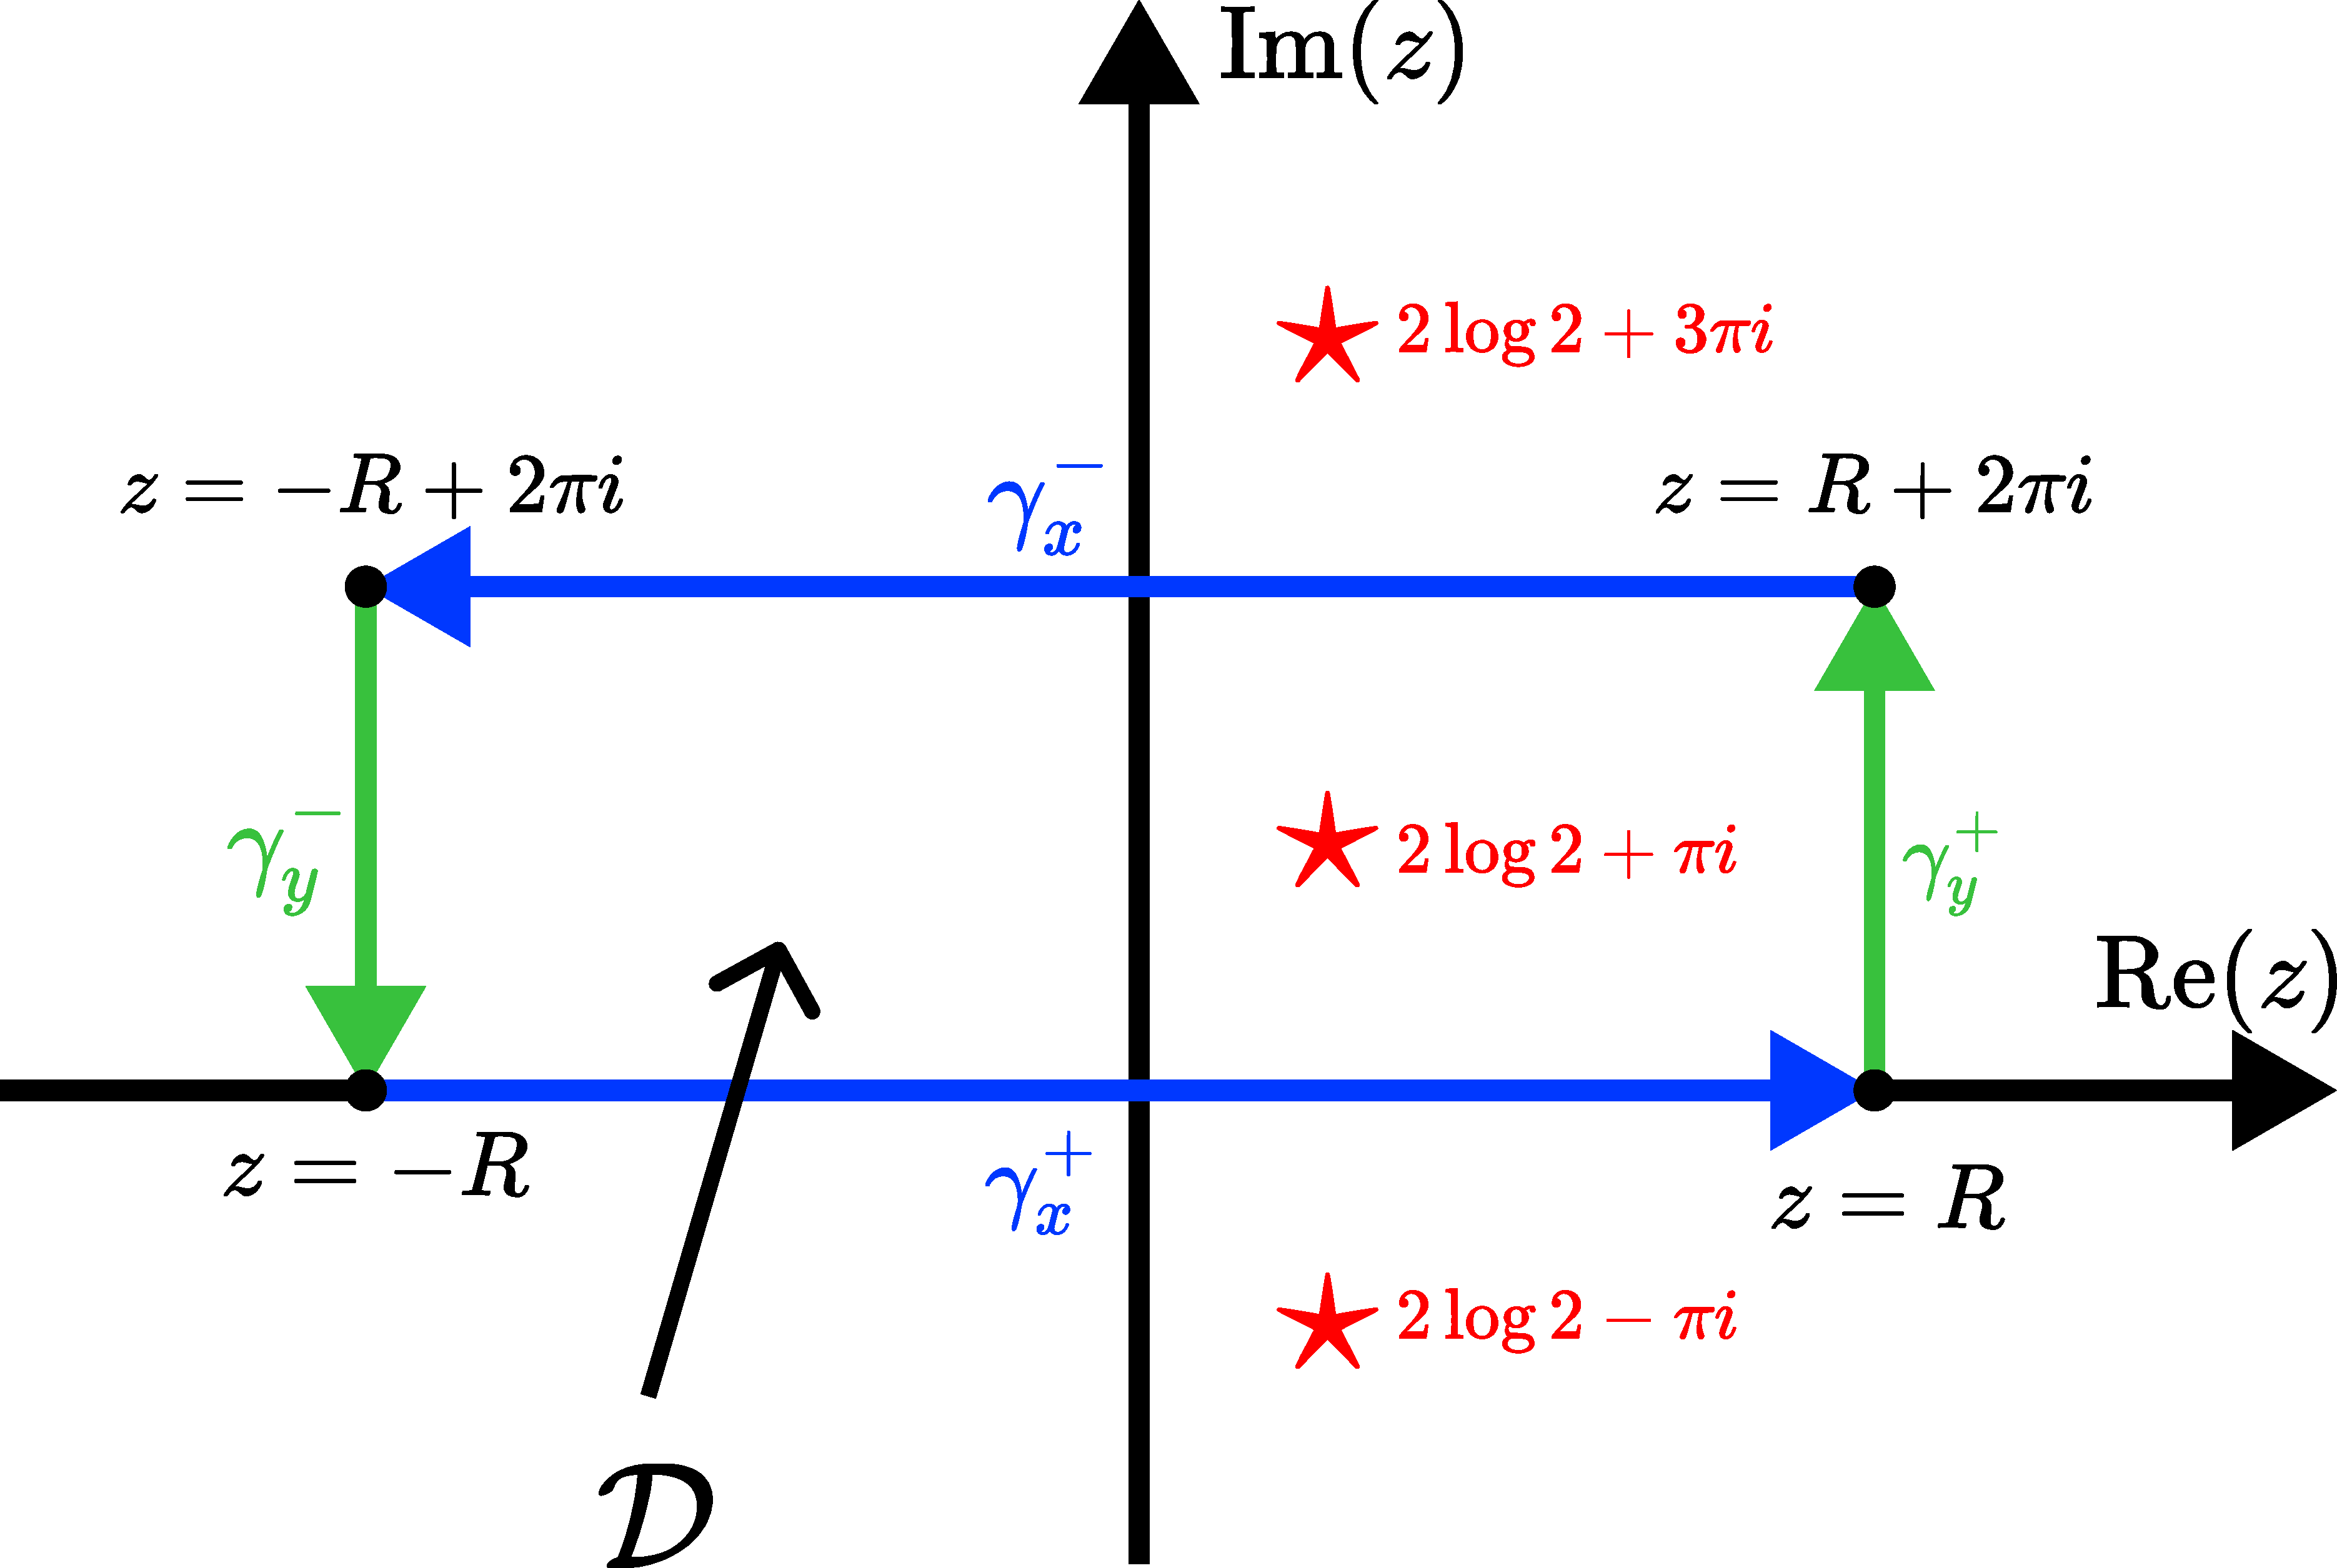
\includegraphics[width=0.6\textwidth]{images/hw_3/contour_2.pdf}
    \caption{Контур $\gamma$ в задачі 2 з особливими точками $f(z)$.}
    \label{fig:contour_2}
\end{figure}

Параметризація на кожному відрізку:
\begin{align}
    &\gamma_x^+: & z = x, & dz = dx & x \in [-R,R] \\
    &\gamma_y^+: & z = R + iy, & dz = idy, & y \in [0,2\pi] \\
    &\gamma_x^-: & z = -x + 2\pi i, & dz = -dx, & x \in [-R,R] \\
    &\gamma_y^-: & z = -R + (2\pi - y)i, & dz = -idy, & y \in [0,2\pi]
\end{align}

Таким чином, маємо:
\begin{equation}\label{eq:1}
    \oint_{\gamma} f(z)dz = \left(\int_{\gamma_x^+} + \int_{\gamma_y^+} + \int_{\gamma_x^-} + \int_{\gamma_y^-}\right)f(z)dz
\end{equation}

Спочатку знайдемо увесь інтеграл $\mathcal{I}_{\gamma} := \oint_{\gamma}f(z)dz$. Для цього помітимо, що всередині контуру лише одна особлива точка $z_0 = 2\log 2 + i\pi$ через вибір висоти в $2\pi$. В такому разі:
\begin{equation*}
    \mathcal{I}_{\gamma} = 2\pi i \cdot \frac{e^{z/4}}{(4+e^z)'}\Big|_{z=2\log 2 + i\pi} = 2\pi i e^{-3z/4}\Big|_{z=2\log 2 + i\pi} = -2\pi i \cdot \frac{1+i}{4} = \frac{\pi(1-i)}{2}
\end{equation*}

Отже, залишилось оцінити чотири інтеграли у правій частині рівняння \ref{eq:1} при прямуванні $R \to \infty$. 

\textbf{Інтеграл по $\gamma_x^+$.} $\int_{\gamma_x^+}f(z)dz = \int_{-R}^{+R}f(x)dx$, тому $\lim_{R \to \infty}\int_{\gamma_x^+}f(z)dz = \mathcal{I}$ -- шуканий інтеграл.

\textbf{Інтеграл по $\gamma_x^-$.} Розпишемо:
\begin{equation}
    \int_{\gamma_x^-}f(z)dz = -\int_{-R}^{+R} \frac{e^{\frac{-x+2\pi i}{4}}}{4+e^{-x+2\pi i}}dx = -i \int_{-R}^R \frac{e^{-\frac{x}{4}}dx}{4+e^{-x}} = -i \int_{-R}^R \frac{e^{\frac{x}{4}}dx}{4+e^{x}}
\end{equation}

З цього можна отримати $\lim_{R \to \infty} \int_{\gamma_x^-}f(z)dz = -i\mathcal{I}$. 

\textbf{Інтеграл по $\gamma_y^+$.} Тут нам треба показати, що $\lim_{R \to \infty}\int_{\gamma_y^+}f(z)dz = 0$. Для цього оцінимо наш інтеграл. Спочатку підставимо $z=R+iy$:
\begin{equation}
    \int_{\gamma_y^+}f(z)dz = i\int_0^{2\pi} \frac{e^{(R+iy)/4}dy}{4+e^{R+iy}} = i \int_0^{2\pi} \frac{e^{R/4}e^{iy/4}dy}{4+e^Re^{iy}}
\end{equation}

Далі починаємо оцінювати:
\begin{equation}
    \left|\int_{\gamma_y^+}f(z)dz\right| \leq 2\pi \sup_{y \in [0,2\pi]} \frac{e^{R/4}|e^{iy/4}|}{|4+e^Re^{iy}|} = 2\pi \sup_{y \in [0,2\pi]} \frac{e^{R/4}}{|4+e^Re^{iy}|}
\end{equation}

Оцінимо знаменник як $|e^Re^{iy} + 4| \geq ||e^Re^{iy}| - 4| = e^R - 4$\footnote{Вважаємо $R$ достатньо великим, так що $e^R > 4$}, тому
\begin{equation}
    \left|\int_{\gamma_y^+}f(z)dz\right| \leq \frac{2\pi e^{R/4}}{e^R - 4} \sim \frac{2\pi}{e^{3R/4}} \xrightarrow[R \to \infty]{} 0 
\end{equation}

Отже $\lim_{R \to \infty}\int_{\gamma_y^+}f(z)dz = 0$. 

\textbf{Інтеграл по $\gamma_y^-$.} Аналогічно покажемо, що $\lim_{R \to \infty}\int_{\gamma_y^-}f(z)dz = 0$. Підставимо $z=-R+(2\pi - y)i$:
\begin{gather}
    \int_{\gamma_y^-}f(z)dz = -i\int_0^{2\pi} \frac{e^{(-R+(2\pi - y)i)/4}dy}{4+e^{-R+(2\pi - y)i}} = -i \int_0^{2\pi} \frac{e^{-R/4}e^{\pi i/2}e^{-iy/4}dy}{4+e^{-R}e^{2\pi i}e^{-iy}} \nonumber \\
    = \int_0^{2\pi} \frac{e^{-R/4}e^{-iy/4}dy}{4+e^{-R}e^{-iy}}
\end{gather}

Отже, модуль:
\begin{equation}
    \left|\int_{\gamma_y^-}f(z)dz\right| \leq 2\pi \sup_{y \in [0,2\pi]} \frac{|e^{-R/4}||e^{-iy/4}|}{|4+e^{-R}e^{-iy}|} = 2\pi \sup_{y \in [0,2\pi]} \frac{e^{-R/4}}{|4+e^{-R}e^{-iy}|}
\end{equation}

Оцінимо знаменник як $|4+e^{-R}e^{-iy}| \geq |4 - |e^{-R}e^{-iy}|| = 4 - e^{-R}$, тому
\begin{equation}
    \left|\int_{\gamma_y^-}f(z)dz\right| \leq \frac{2\pi e^{-R/4}}{4-e^{-R}} \xrightarrow[R \to \infty]{} 0
\end{equation}

Таким чином $\lim_{R \to \infty}\int_{\gamma_y^-}f(z)dz = 0$.

Остаточно маємо:
\begin{equation}
    \mathcal{I}_{\gamma} = \mathcal{I} - i\mathcal{I} \implies \mathcal{I} = \frac{\mathcal{I}_{\gamma}}{1-i} = \boxed{\frac{\pi}{2}}
\end{equation}

\textbf{Відповідь.} $\frac{\pi}{2}$. 

\problem{}

\textbf{Умова.} Обчислити інтеграл
\begin{equation*}
    \mathcal{I} = \int_{0}^{+\infty} \frac{\log x }{x^2+5}dx
\end{equation*}

\textbf{Розв'язання.} Оскільки розглядання функції $f(z) = \frac{\text{Log}(z)}{z^2+5}$ тут слабо допоможе, то замість цього будемо розглядати функцію 
\begin{equation}
    f(z) = \frac{\text{Log}^2(z)}{z^2+5}
\end{equation}

Далі оберемо контур (див. Рисунок \ref{fig:contour_3})
\begin{equation}
    \Gamma_{\varepsilon, R} = C_R \cup C_{\epsilon} \cup \underbrace{[\varepsilon, R]}_{\text{двічі}}
\end{equation}

\begin{figure}
    \centering
    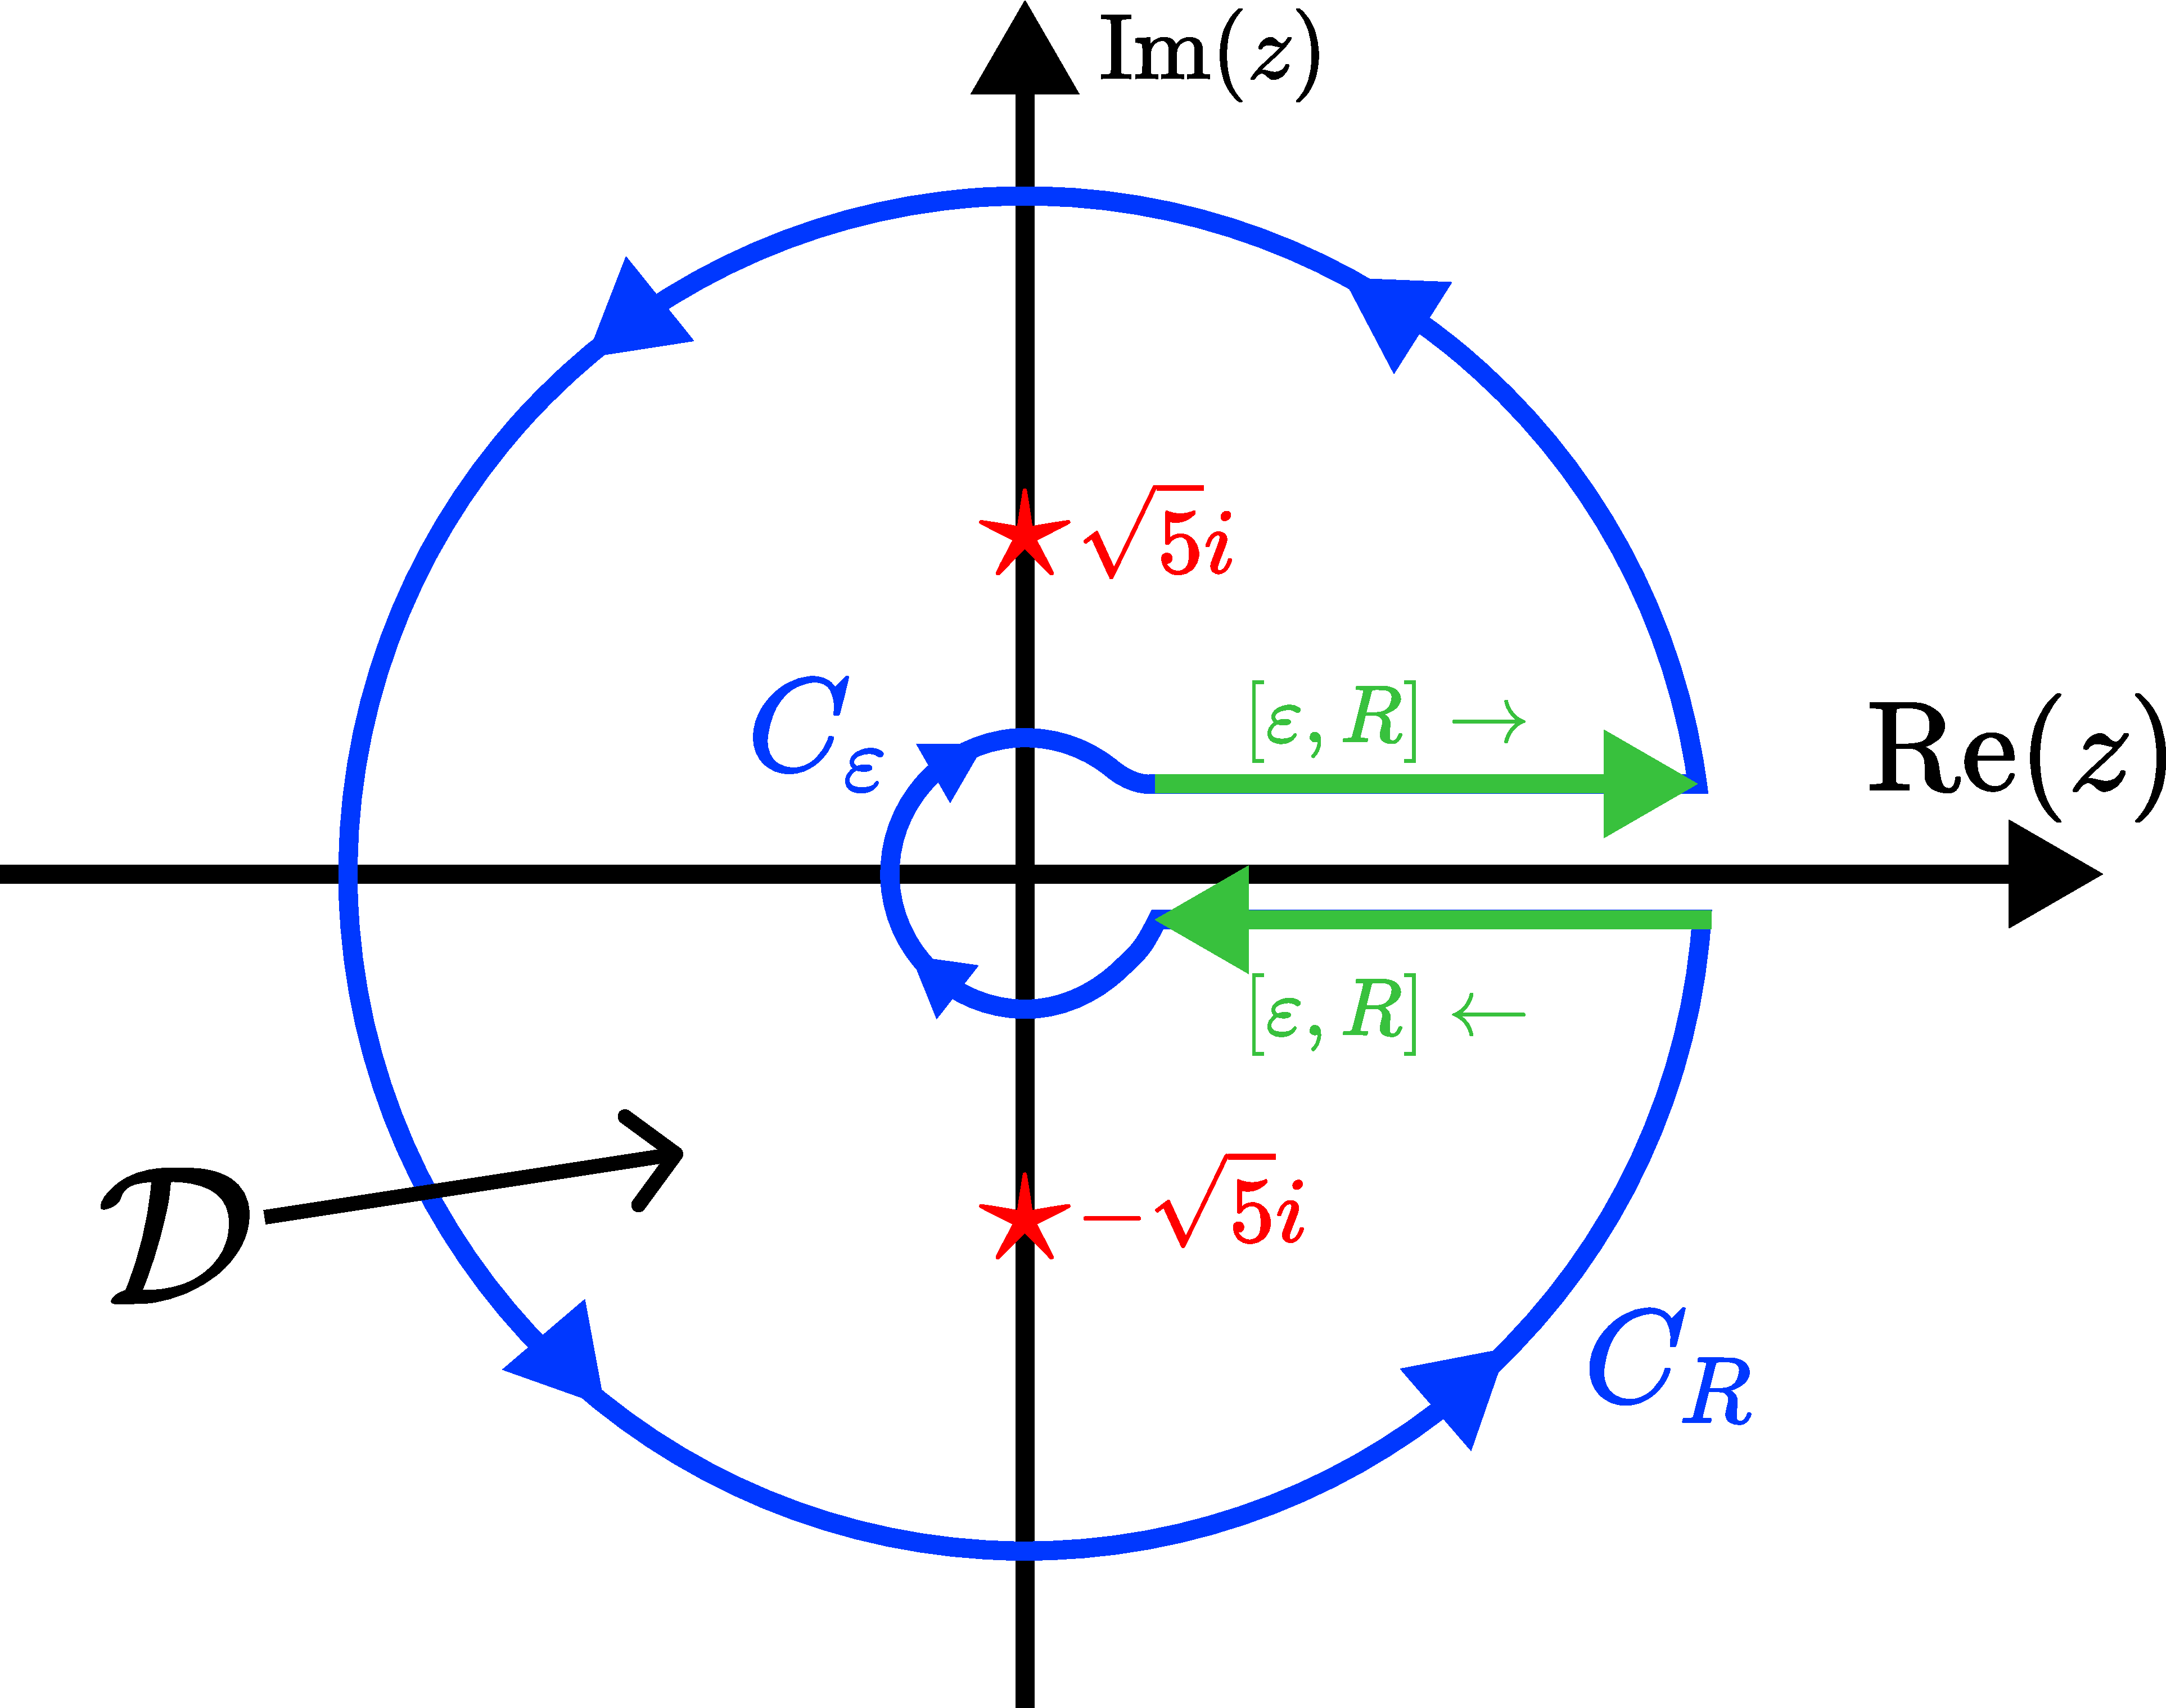
\includegraphics[width=0.6\textwidth]{images/hw_3/contour_3.pdf}
    \caption{Контур $\gamma$ в задачі 3 з особливими точками $f(z)$.}
    \label{fig:contour_3}
\end{figure}

Отже, запишемо інтеграл по $\Gamma_{\varepsilon, R}$:
\begin{equation*}
    \oint_{\Gamma_{\varepsilon, R}} f(z)dz = \int_{\varepsilon}^R \frac{\ln^2 x dx}{x^2+5} + \int_{C_R}f(z)dz - \int_{\varepsilon}^R \frac{(\ln x + 2\pi i)^2dx}{x^2+5} + \int_{C_{\varepsilon}}f(z)dz
\end{equation*}

Далі ми покажемо, що $\lim_{R \to \infty}\int_{C_R}f(z)dz = \lim_{\varepsilon \to 0}\int_{C_{\varepsilon}}f(z)dz = 0$, а інтеграл $\lim_{\varepsilon \to 0, R \to \infty}\int_{\varepsilon}^R \frac{\ln^2 x dx}{x^2+5} = \mathcal{I}$ -- шуканий. Тому поки не зрозуміло, що робити з третім інтегралом в правій частині. Тому, розпишемо його:

\begin{equation}
    \int_{\varepsilon}^R \frac{(\ln x + 2\pi i)^2dx}{x^2+5} = \int_{\varepsilon}^R \frac{\ln^2 x dx}{x^2+5} + \int_{\varepsilon}^R \frac{4\pi i \ln x dx}{x^2+5} - \int_{\varepsilon}^R \frac{4\pi^2 dx}{x^2+5}
\end{equation}

Перший інтеграл праворуч пізніше скоротиться, а другий є шуканим при $\varepsilon \to 0, R \to \infty$. Залишається розібратися з інтегралом праворуч. Хоча його не обов'язоково зараз обчислювати (в кінці можна буде уникнути цього, скориставшись системою рівнянь), ми для зручності це зробимо, бо він є стандартним:
\begin{equation}
    \lim_{\varepsilon \to 0, R \to \infty}\int_{\varepsilon}^R \frac{4\pi^2 dx}{x^2+5} = 4\pi^2 \int_{0}^{+\infty} \frac{dx}{x^2+5} = \frac{4\pi^2}{\sqrt{5}}\arctan \frac{x}{\sqrt{5}}\Big|_{x \to 0}^{x \to +\infty} = \frac{2\pi^3}{\sqrt{5}}
\end{equation}

Отже, повернемось до нашого початкового інтегралу:
\begin{gather}
    \oint_{\Gamma_{\varepsilon, R}} f(z)dz = \int_{C_R}f(z)dz + \int_{C_{\varepsilon}}f(z)dz + \int_{\varepsilon}^R \frac{\ln^2 xdx}{x^2+5} \nonumber \\
    - \int_{\varepsilon}^R \frac{\ln^2 x dx}{x^2+5} - 4\pi i \int_{\varepsilon}^R \frac{\ln x dx}{x^2+5} + 4\pi^2\int_{\varepsilon}^R \frac{dx}{x^2+5}
\end{gather}

Бачимо, що дійсно $\int_{\varepsilon}^R \frac{\ln^2 xdx}{x^2+5}$ скоротилося, а при переході $\varepsilon \to 0, R \to \infty$ маємо:
\begin{gather}
    \oint_{\Gamma_{\varepsilon, R}} f(z)dz = -4\pi i \cdot  \mathcal{I} + \frac{2\pi^3}{\sqrt{5}}
\end{gather}

Отже, наш розв'язок зводиться до трьох кроків: оцінці інтегралу по $C_R$, по $C_{\varepsilon}$, а також обрахунок $\oint_{\Gamma_{\varepsilon, R}}f(z)dz$. 

\textbf{Обрахунок інтеграла по $\Gamma_{\varepsilon, R}$.} Дві особливі точки функції $f(z) = \frac{\text{Log}^2(z)}{z^2+5}$ є $z=\pm \sqrt{5}i$ -- обидві лежать всередині контуру і є полюсами першого порядку. Таким чином,
\begin{equation}
    \oint_{\Gamma_{\varepsilon, R}} f(z)dz = 2\pi i\left(\text{Res}_{z=\sqrt{5}i}f(z) + \text{Res}_{z=-\sqrt{5}i}f(z)\right)
\end{equation}

Тепер обраховуємо лишки:
\begin{gather}
    \text{Res}_{z=\sqrt{5}i}f(z) = \frac{\text{Log}^2(z)}{(z^2+5)'}\Big|_{z=\sqrt{5}i} = \frac{\text{Log}^2(\sqrt{5}i)}{2\sqrt{5}i} = \frac{(\log \sqrt{5} + i\cdot \text{arg}(i\sqrt{5}))^2}{2\sqrt{5}i} \nonumber \\
    = \frac{(\log \sqrt{5} + i \cdot \frac{\pi}{2})^2}{2\sqrt{5}i} = \frac{\log^2 \sqrt{5}}{2\sqrt{5}i} + \frac{2\log\sqrt{5} \cdot i \pi}{2\cdot 2\sqrt{5}i} - \frac{\pi^2}{4 \cdot 2\sqrt{5}i} \nonumber \\
    = \frac{\log^2 5 - \pi^2}{8\sqrt{5}i} + \frac{\pi \log 5}{4\sqrt{5}}
\end{gather}

Другий лишок:
\begin{gather}
    \text{Res}_{z=-\sqrt{5}i}f(z) = \frac{\text{Log}^2(z)}{(z^2+5)'}\Big|_{z=-\sqrt{5}i} = -\frac{(\log \sqrt{5} + \frac{3\pi i}{2})^2}{2\sqrt{5}i} \nonumber \\
    = -\frac{\log^2 \sqrt{5}}{2\sqrt{5}i} - \frac{3\pi i \log \sqrt{5}}{2\sqrt{5}i} + \frac{9\pi^2}{4 \cdot 2\sqrt{5}i} \nonumber \\
    = \frac{-\log^2 5 + 9\pi^2}{8\sqrt{5}i} - \frac{3\pi \log 5}{4\sqrt{5}}
\end{gather}

Таким чином, інтеграл:
\begin{equation}
    \oint_{\Gamma_{\varepsilon, R}} f(z)dz = 2\pi i \left(\frac{\pi^2}{\sqrt{5}i} - \frac{\pi \log 5}{2\sqrt{5}}\right) = \frac{2\pi^3}{\sqrt{5}} - \frac{\pi^2 \log 5}{\sqrt{5}}i
\end{equation}

Таким чином, можемо знайти наш шуканий інтеграл:
\begin{equation}
    \frac{2\pi^3}{\sqrt{5}} - \frac{\pi^2\log 5}{\sqrt{5}}i = -4\pi i \cdot \mathcal{I} + \frac{2\pi^3}{\sqrt{5}} \implies \mathcal{I} = \frac{\pi^2 \log 5}{4\pi\sqrt{5}} = \boxed{\frac{\pi \log 5}{4\sqrt{5}}}
\end{equation}

\textbf{Оцінка інтегралу по $C_R$}. Тепер покажемо, що $\lim_{R \to \infty}\int_{C_R}f(z)dz = 0$. Починаємо робити оцінку:
\begin{equation}
    \left|\int_{C_R}f(z)dz\right| \leq 2\pi R \sup_{z \in C_R} \frac{|\text{Log}^2(z)|}{|z^2+5|} \leq \frac{2\pi R(\log^2 R + 4\pi^2)}{R^2 - 5} \xrightarrow[R \to \infty]{} 0
\end{equation}

\textbf{Оцінка інтегралу по $C_{\varepsilon}$}. Тепер покажемо, що $\lim_{\varepsilon \to 0}\int_{C_{\varepsilon}}f(z)dz = 0$. Знову робимо оцінку:
\begin{equation}
    \left|\int_{C_{\varepsilon}}f(z)dz\right| \leq 2\pi \varepsilon \sup_{z \in C_{\varepsilon}} \frac{|\text{Log}^2(z)|}{|z^2+5|} \leq \frac{2\pi \varepsilon(\log^2 \varepsilon + 4\pi^2)}{5 - \varepsilon^2} \xrightarrow[\varepsilon \to 0]{} 0
\end{equation}

Отже, остаточно $\boxed{\mathcal{I} = \frac{\pi \log 5}{4\sqrt{5}}}$.

\textbf{Відповідь.} $\frac{\pi \log 5}{4\sqrt{5}}$.

\end{document}
